\chapter{Исследовательская часть}

\section{Технические характеристики}
Технические характеристики устройства, на котором выполнялись
замеры по времени:

\begin{itemize}
    \item Процессор: Intel Core i7 9750H 2.6 ГГц;
    \item Оперативная память: 16 ГБ;
    \item Операционная система: Kubuntu 22.04.3 LTS x86\_64 Kernel: 6.2.0-36-generic
\end{itemize}

Во время проведения измерений времени ноутбук был подключен к сети электропитания и был нагружен только системными приложениями.

\section{Демонстрация работы программы}

На рисунке \ref{fig:img_prog} показан пример работы с программой.


\begin{figure}[ht!]
	\centering
	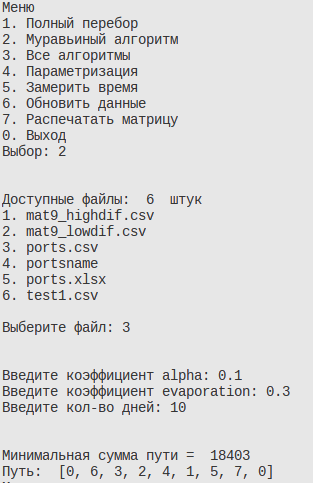
\includegraphics[width=170mm]{inc/img/img_prog.png}
	\caption{Демонстрация работы программы.\label{overflow}}
	\label{fig:img_prog}
	\end{figure}


\clearpage

\section{Временные характеристики}

Для замера процессорного времени используется функция \textit{process\_time()} из библиотеки \textit{time} на \textit{Python}. Функция возвращает процессорное время типа float в секундах.

Использовать функцию приходится дважды, затем из конечного времени нужно вычесть начальное, чтобы получить результат.

Замеры проводились для разного размера матриц, чтобы определить, когда наиболее эффективно использовать муравьиный алгоритм.

Результаты замеров приведены в таблице \ref{tbl:time_mes} (время в с).


\begin{center}
	\captionsetup{justification=raggedright,singlelinecheck=off}
	\begin{longtable}[c]{|p{4cm}|p{4cm}|p{4cm}|}
		\caption{Результаты замеров времени\label{tbl:time_mes}}\\ \hline
		Размер & Полный перебор & Муравьиный \\ \hline
		2 &   0.000130 &   0.019932 \\ \hline
		3 &   0.000138 &   0.031615 \\ \hline
		4 &   0.000104 &   0.044361 \\ \hline
		5 &   0.000420 &   0.089291 \\ \hline
		6 &   0.002390 &   0.152131 \\ \hline
		7 &   0.019703 &   0.254059 \\ \hline
		8 &   0.162850 &   0.398472 \\ \hline
		9 &   1.637611 &   0.594024 \\ \hline
		10 &  18.207853 &   0.857666 \\ \hline
	\end{longtable}
\end{center}

\clearpage

Также на рисунке \ref{graph:graph_alg} приведены графические результаты замеров.

\begin{figure}[ht!]
	\centering
	\includesvg[width=1.0\textwidth]{inc/img/plotting_data1.svg}
	\caption{Сравнение по времени алгоритмов полного перебора путей и муравьиного на разных размерах матриц\label{graph:graph_alg}}
	\label{fig:plotting_data1}
	\end{figure}


% \begin{figure}[ht!]
% 	\begin{center}
% 		\captionsetup{singlelinecheck = false, justification=centerfirst}
% 		\begin{tikzpicture}
% 			\begin{axis}[
% 				xlabel={Размер матрицы},
% 				ylabel={время, с},
% 				width = 0.95\textwidth,
% 				height=0.3\textheight,
% 				xmin=2, xmax=11,
% 				legend pos=north west,
% 				xmajorgrids=true,
% 				grid style=dashed,
% 				]
% 				\addplot[
% 				red,
% 				semithick,
% 				mark = *,
% 				mark size = 5pt,
% 				thick,
% 				] file {assets/time.dat};
% 				\addplot[
% 				blue,
% 				semithick,
% 				mark = x,
% 				mark size = 5pt,
% 				thick,
% 				] file {assets/time2.dat};
				
% 				\legend{
% 					Полный перебор,
% 					Муравьиный алгоритм,
% 				}
% 			\end{axis}
% 		\end{tikzpicture}
% 		\centering
% 		\caption{Сравнение по времени алгоритмов полного перебора путей и муравьиного на разных размерах матриц}
% 		\label{graph:graph_alg}
% 	\end{center}
	
% \end{figure}

\clearpage


\section{Постановка исследования}

Автоматическая параметризация была проведена на двух классах данных --- \ref{par:class1} и \ref{par:class2}. Алгоритм будет запущен для набора значений $\alpha, \rho \in (0, 1)$.

Итоговая таблица значений параметризации будет состоять из следующих колонок:
\begin{itemize}[label=---]
	\item $\alpha$ --- коэффициент жадности;
	\item $\rho$ --- коэффициент испарения;
	\item \textit{days} --- количество дней жизни колонии муравьёв;
	\item \textit{Result} --- эталонный результат, полученный методом полного перебора для проведения данного исследования;
	\item \textit{Mistake} --- разность полученного основаным на муравьином алгоритме методом значения и эталонного значения на данных значениях параметров, показатель качества решения.
\end{itemize}

\textit{Цель исследования} --- определить комбинацию параметров, которые позволяют решаить задачу наилучшим образом для выбранного класса данных. Качество решения зависит от количества дней и погрешности измерений.


\subsection{Класс данных 1}
\label{par:class1}

Класс данных 1 представляет собой матрицу смежности размером 9 элементов (небольшой разброс значений --- от 1 до 2), которая представлена далее.

\begin{equation}
	\label{eq:kd1}
	K_{1} = \begin{pmatrix}
		0 & 1 & 1 & 2 & 2 & 1 & 1 & 1 & 2 \\ 
		1 & 0 & 1 & 2 & 1 & 1 & 2 & 1 & 1 \\ 
		1 & 1 & 0 & 2 & 2 & 1 & 1 & 2 & 2 \\ 
		2 & 2 & 2 & 0 & 1 & 2 & 1 & 2 & 2 \\ 
		2 & 1 & 2 & 1 & 0 & 2 & 2 & 1 & 1 \\ 
		1 & 1 & 1 & 2 & 2 & 0 & 1 & 1 & 2 \\ 
		1 & 2 & 1 & 1 & 2 & 1 & 0 & 2 & 2 \\ 
		1 & 1 & 2 & 2 & 1 & 1 & 2 & 0 & 2 \\ 
		2 & 1 & 2 & 2 & 1 & 2 & 2 & 2 & 0 
	\end{pmatrix}
\end{equation}

Для данного класса данных приведена таблица \ref{tbl:table_kd1}	с выборкой параметров, которые наилучшим образом решают поставленную задачу, полные результаты параметризации приведены в приложении А. Использованы следующие обозначения: Days --- количество дней, Result --- результат работы, Mistake --- ошибка как отклонение решения от эталонного .

\begin{center}
	\captionsetup{justification=raggedright,singlelinecheck=off}
	\begin{longtable}[c]{|c|c|c|c|c|}
		\caption{Параметры для класса данных 1\label{tbl:table_kd1}}\\ \hline
		$\alpha$ & $\rho$ & Days & Result & Mistake \\ \hline
		0.1 & 0.3 &  10 &    9 &    0 \\
		0.1 & 0.3 &  50 &    9 &    0 \\
		0.1 & 0.3 & 100 &    9 &    0 \\
		0.1 & 0.3 & 300 &    9 &    0 \\
		0.1 & 0.3 & 500 &    9 &    0 \\ \hline
		0.1 & 0.4 &  10 &    9 &    0 \\
		0.1 & 0.4 &  50 &    9 &    0 \\
		0.1 & 0.4 & 100 &    9 &    0 \\
		0.1 & 0.4 & 300 &    9 &    0 \\
		0.1 & 0.4 & 500 &    9 &    0 \\ \hline
		0.1 & 0.7 &  10 &    9 &    0 \\
		0.1 & 0.7 &  50 &    9 &    0 \\
		0.1 & 0.7 & 100 &    9 &    0 \\
		0.1 & 0.7 & 300 &    9 &    0 \\
		0.1 & 0.7 & 500 &    9 &    0 \\ \hline
		0.2 & 0.5 &  10 &    9 &    0 \\
		0.2 & 0.5 &  50 &    9 &    0 \\
		0.2 & 0.5 & 100 &    9 &    0 \\
		0.2 & 0.5 & 300 &    9 &    0 \\
		0.2 & 0.5 & 500 &    9 &    0 \\ \hline
		0.2 & 0.7 &  10 &    9 &    0 \\
		0.2 & 0.7 &  50 &    9 &    0 \\
		0.2 & 0.7 & 100 &    9 &    0 \\
		0.2 & 0.7 & 300 &    9 &    0 \\
		0.2 & 0.7 & 500 &    9 &    0 \\ \hline
		0.3 & 0.4 &  10 &    9 &    0 \\
		0.3 & 0.4 &  50 &    9 &    0 \\
		0.3 & 0.4 & 100 &    9 &    0 \\
		0.3 & 0.4 & 300 &    9 &    0 \\
		0.3 & 0.4 & 500 &    9 &    0 \\ \hline
		0.3 & 0.5 &  10 &    9 &    0 \\
		0.3 & 0.5 & 100 &    9 &    0 \\
		0.3 & 0.5 & 300 &    9 &    0 \\
		0.3 & 0.5 & 500 &    9 &    0 \\ \hline
		0.4 & 0.5 &  10 &    9 &    0 \\
		0.4 & 0.5 &  50 &    9 &    0 \\
		0.4 & 0.5 & 100 &    9 &    0 \\
		0.4 & 0.5 & 300 &    9 &    0 \\
		0.4 & 0.5 & 500 &    9 &    0 \\ \hline
		0.6 & 0.1 &  10 &    9 &    0 \\
		0.6 & 0.1 &  50 &    9 &    0 \\
		0.6 & 0.1 & 100 &    9 &    0 \\
		0.6 & 0.1 & 300 &    9 &    0 \\
		0.6 & 0.1 & 500 &    9 &    0 \\ \hline
	\end{longtable}
\end{center}


\subsection{Класс данных 2}\label{par:class2}


Класс данных 2 представляет собой матрицу смежности размером 9 элементов (большой разброс значений - от 1000 до 9999), которая представлена далее.

\begin{equation}
	\label{eq:kd2}
	K_{1} = \begin{pmatrix}
		0 & 9271 & 8511 & 2010 & 1983 & 7296 & 7289 & 3024 & 1011 \\
		9271 & 0 & 7731 & 4865 & 5494 & 6812 & 4755 & 7780 & 7641 \\
		8511 & 7731 & 0 & 1515 & 9297 & 7506 & 5781 & 5804 & 7334 \\
		2010 & 4865 & 1515 & 0 & 3662 & 9597 & 2876 & 8188 & 9227 \\
		1983 & 5494 & 9297 & 3662 & 0 & 8700 & 4754 & 7445 & 3834 \\
		7296 & 6812 & 7506 & 9597 & 8700 & 0 & 4216 & 5553 & 8215 \\
		7289 & 4755 & 5781 & 2876 & 4754 & 4216 & 0 & 4001 & 4715 \\
		3024 & 7780 & 5804 & 8188 & 7445 & 5553 & 4001 & 0 & 9522 \\
		1011 & 7641 & 7334 & 9227 & 3834 & 8215 & 4715 & 9522 & 0 
	\end{pmatrix}
\end{equation}


Для данного класса данных приведена таблица с выборкой параметров, которые наилучшим образом решают поставленную задачу Days --- количество дней, Result --- результат работы, Mistake --- ошибочность полученного результата).

\begin{center}
	\captionsetup{justification=raggedright,singlelinecheck=off}
	\begin{longtable}[c]{|c|c|c|c|c|}
		\caption{Параметры для класса данных 2\label{tbl:table_kd2}}\\ \hline
		$\alpha$ & $\rho$ & Days & Result & Mistake \\ \hline
		0.1 &  0.3 &  100 & 34192 &     0 \\
		0.1 &  0.3 &  300 & 34192 &     0 \\
		0.1 &  0.3 &  500 & 34192 &     0 \\ \hline
		0.1 &  0.7 &  100 & 34192 &     0 \\
		0.1 &  0.7 &  300 & 34192 &     0 \\
		0.1 &  0.7 &  500 & 34192 &     0 \\ \hline
		0.2 &  0.1 &  100 & 34192 &     0 \\
		0.2 &  0.1 &  300 & 34192 &     0 \\
		0.2 &  0.1 &  500 & 34192 &     0 \\ \hline
		0.2 &  0.2 &  100 & 34192 &     0 \\
		0.2 &  0.2 &  300 & 34192 &     0 \\
		0.2 &  0.2 &  500 & 34192 &     0 \\ \hline
		0.2 &  0.5 &  100 & 34192 &     0 \\
		0.2 &  0.5 &  300 & 34192 &     0 \\
		0.2 &  0.5 &  500 & 34192 &     0 \\ \hline
		0.2 &  0.8 &  100 & 34192 &     0 \\
		0.2 &  0.8 &  300 & 34192 &     0 \\
		0.2 &  0.8 &  500 & 34192 &     0 \\ \hline
		0.3 &  0.1 &  100 & 34192 &     0 \\
		0.3 &  0.1 &  300 & 34192 &     0 \\
		0.3 &  0.1 &  500 & 34192 &     0 \\ \hline
		0.3 &  0.2 &    5 & 34192 &     0 \\
		0.3 &  0.2 &   50 & 34192 &     0 \\
		0.3 &  0.2 &  100 & 34192 &     0 \\
		0.3 &  0.2 &  300 & 34192 &     0 \\
		0.3 &  0.2 &  500 & 34192 &     0 \\ \hline
		0.4 &  0.5 &   50 & 34192 &     0 \\
		0.4 &  0.5 &  300 & 34192 &     0 \\
		0.4 &  0.5 &  500 & 34192 &     0 \\ \hline
		0.5 &  0.2 &  100 & 34192 &     0 \\
		0.5 &  0.2 &  300 & 34192 &     0 \\
		0.5 &  0.2 &  500 & 34192 &     0 \\ \hline
		0.6 &  0.2 &  100 & 34192 &     0 \\
		0.6 &  0.2 &  300 & 34192 &     0 \\
		0.6 &  0.2 &  500 & 34192 &     0 \\ \hline
		0.6 &  0.3 &  300 & 34192 &     0 \\
		0.6 &  0.3 &  500 & 34192 &     0 \\ \hline
		0.6 &  0.4 &  100 & 34192 &     0 \\
		0.6 &  0.4 &  500 & 34192 &     0 \\ \hline
		0.6 &  0.5 &  100 & 34192 &     0 \\
		0.6 &  0.5 &  300 & 34192 &     0 \\
		0.6 &  0.5 &  500 & 34192 &     0 \\ \hline
	\end{longtable}
\end{center}

\subsection{Класс данных 3}
\label{par:class3}

Класс данных 3 представляет собой матрицу смежности расстояний между следующими портами: Новороссийск, Усть-Луга, Восточный, Приморск, Санкт-Петербург, Мурманск, Порт-Кавказ, Ванино\cite{dist}.

\begin{equation}
	\label{eq:kd3}
	K_{3} = \begin{pmatrix}
		0 & 4525 & 5112 & 160 & 4581 & 5074 & 513 & 9686 \\ 
		4525 & 0 & 417 & 4682 & 67 & 2092 & 4479 & 12840 \\ 
		5112 & 417 & 0 & 613 & 349 & 2492 & 5095 & 13250 \\ 
		160 & 4682 & 613 & 0 & 4729 & 5221 & 84 & 9826 \\ 
		4581 & 67 & 349 & 4729 & 0 & 2083 & 4745 & 12900 \\ 
		5074 & 2092 & 2492 & 5221 & 2083 & 0 & 4978 & 4999 \\ 
		513 & 4479 & 5095 & 84 & 4745 & 4978 & 0 & 9734 \\ 
		9686 & 12840 & 13250 & 9826 & 12900 & 4999 & 9734 & 0
	\end{pmatrix}
\end{equation}

\begin{center}
	\captionsetup{justification=raggedright,singlelinecheck=off}
	\begin{longtable}[c]{|c|c|c|c|c|}
		\caption{Параметры для класса данных 3\label{tbl:table_kd3}}\\ \hline
		$\alpha$ & $\rho$ & Days & Result & Mistake \\ \hline
		0.1 &  0.3 &  100 & 18403 &     0 \\
		0.1 &  0.3 &  300 & 18403 &     0 \\
		0.1 &  0.3 &  500 & 18403 &     0 \\ \hline
		0.1 &  0.7 &  100 & 18403 &     0 \\
		0.1 &  0.7 &  300 & 18403 &     0 \\
		0.1 &  0.7 &  500 & 18403 &     0 \\ \hline
		0.2 &  0.1 &  100 & 18403 &     0 \\
		0.2 &  0.1 &  300 & 18403 &     0 \\
		0.2 &  0.1 &  500 & 18403 &     0 \\ \hline
		0.2 &  0.2 &  100 & 18403 &     0 \\
		0.2 &  0.2 &  300 & 18403 &     0 \\
		0.2 &  0.2 &  500 & 18403 &     0 \\ \hline
		0.2 &  0.5 &  100 & 18403 &     0 \\
		0.2 &  0.5 &  300 & 18403 &     0 \\
		0.2 &  0.5 &  500 & 18403 &     0 \\ \hline
		0.2 &  0.8 &  100 & 18403 &     0 \\
		0.2 &  0.8 &  300 & 18403 &     0 \\
		0.2 &  0.8 &  500 & 18403 &     0 \\ \hline
		0.3 &  0.1 &  100 & 18403 &     0 \\
		0.3 &  0.1 &  300 & 18403 &     0 \\
		0.3 &  0.1 &  500 & 18403 &     0 \\ \hline
		0.3 &  0.2 &    5 & 18403 &     0 \\
		0.3 &  0.2 &   50 & 18403 &     0 \\
		0.3 &  0.2 &  100 & 18403 &     0 \\
		0.3 &  0.2 &  300 & 18403 &     0 \\
		0.3 &  0.2 &  500 & 18403 &     0 \\ \hline
		0.4 &  0.5 &   50 & 18403 &     0 \\
		0.4 &  0.5 &  300 & 18403 &     0 \\
		0.4 &  0.5 &  500 & 18403 &     0 \\ \hline
		0.5 &  0.2 &  100 & 18403 &     0 \\
		0.5 &  0.2 &  300 & 18403 &     0 \\
		0.5 &  0.2 &  500 & 18403 &     0 \\ \hline
		0.6 &  0.2 &  100 & 18403 &     0 \\
		0.6 &  0.2 &  300 & 18403 &     0 \\
		0.6 &  0.2 &  500 & 18403 &     0 \\ \hline
		0.6 &  0.3 &  300 & 18403 &     0 \\
		0.6 &  0.3 &  500 & 18403 &     0 \\ \hline
		0.6 &  0.4 &  100 & 18403 &     0 \\
		0.6 &  0.4 &  500 & 18403 &     0 \\ \hline
		0.6 &  0.5 &  100 & 18403 &     0 \\
		0.6 &  0.5 &  300 & 18403 &     0 \\
		0.6 &  0.5 &  500 & 18403 &     0 \\ \hline
	\end{longtable}
\end{center}

\section*{Вывод}

В результате исследования было получно, что использование муравьиного алгоритма наиболее эффективно при больших размерах матриц. Так, при размере матрицы, равном 2, муравьиный алгоритм медленее алгоритма полного перебора в 153 раза, а при размере матрицы, равном 9, муравьиный алгоритм быстрее алгоритма полного перебора в раз, а при размере в 10 -- уже в 21 раз. Следовательно, при рамзерах матриц больше 8 следует использовать муравьиный алгоритм, но стоит учитывать, что он не гарантирует получения глобального оптимума при решении задачи.

Для класса данных 3 (см. п. \ref{par:class3}) было получено, что наилучшим образом алгоритм работает на значениях параметров, которые представлены далее:
\begin{itemize}[label=---]
	\item $\alpha = 0.1, \rho = 0.3, 0.7$;
	\item $\alpha = 0.2, \rho = 0.1, 0.2, 0.5, 0.8$;
	\item $\alpha = 0.3, \rho = 0.1, 0.2$;
	\item $\alpha = 0.4, \rho = 0.5$;
	\item $\alpha = 0.5, \rho = 0.2$;
	\item $\alpha = 0.6, \rho = 0.2, 0.3, 0.4$.
\end{itemize} 
Для этого класса данных рекомендуется использовать данные параметры.

Также во время ислледования было замечено --- чем меньше $\alpha$, тем меньше погрешностей возникает. При этом число дней жизни колонии значительно влияет на качество решения: чем значение параметра $Days$ больше, тем меньше отклонение решения от эталонного.